Die Verknüpfung zwischen Onlinehandel und Onlinemarketing, besonders in der Wirtschaft, wird als E-Commerce bezeichnet. Der E-Commerce ist das Zusammenspiel als auch Resultat der beiden Gebiete. Schon seit an Beginn des Handels selbst ist Werbung untrennbar mit Handel verknüpft. Schon in der Antike haben römische Händler auf ihren Werken Zeichen eingraviert um die Echtheit eines Gegenstandes bewiesen zu können als auch ihren Namen oder Künstlernamen in der Welt zu verbreiten.

\begin{figure}[h]
    \begin{center}
        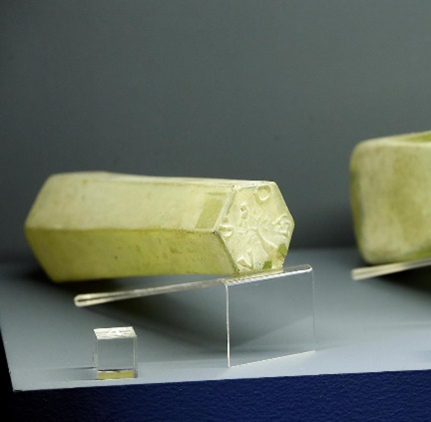
\includegraphics[width=8cm]{media/5.png}
        \caption{Werbung im alten Rom}
        \label{werbung-rom}
        \bildquelle So funktionierte Werbung im alten Rom. In: Welt.de (2019). https://bit.ly/3mRhblX. – aufgerufen am 25. 12. 2020

    \end{center}
\end{figure}
